\chapter{Evaluation perspective on projected shifted partial derivatives}

The measure used in the lower bounds of Kayal, Limaye, Saha, Srinivasan~\cite{KLSS} and Kumar, Saraf~\cite{KS14} was the dimension of projected shifted partials.
As seen in that chapter, the calculations are extremely delicate.
In this chapter, we shall some slight modifications of this measure that is in a sense more \emph{algebraic} and hence useful in other lower bounds. 

\section{Coefficients vs evaluations}

For a moment, let us revisit the lower bounds of Nisan and Wigderson~\cite{nw1997}. The measure studied for the class of homogeneous depth-$3$ circuits in \autoref{thm:low-rank-sps-lb} was the dimension of partial derivatives. 
\[
\CM{NW}_k(f) \spaced{:=} \dim\set{\partial^{=k}(f)}
\]
More precisely, we interpret any element of $\partial^{=k}(f)$ as a long vector of coefficients and look at the dimension of this collection of vectors. That is, $\CM{NW}_k(f)$ is the rank of the following matrix. 

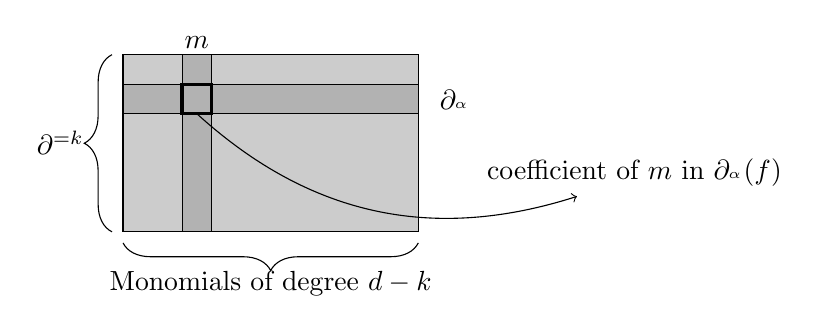
\begin{tikzpicture}[scale=0.75]
\draw[fill=black!20] (0,0) rectangle (5,3);

\draw[decorate,decoration={brace,amplitude=10pt,raise=4pt},yshift=0pt]
(0,0) -- (0,3);
\node[anchor=east] at (-0.5,1.5) {$\partial^{=k}$};
\draw[decorate,decoration={brace,amplitude=10pt,mirror, raise=4pt},yshift=0pt] 
(0,0) -- (5,0);
\node[anchor=north] at (2.5,-0.5) {Monomials of degree $d - k$};

\draw[fill=black!30] (1,0) rectangle (1.5,3);
\node at (1.25,3.2) {$m$};

\draw[fill=black!30] (0,2) rectangle (5,2.5);
\node[anchor=west] at (5.2,2.2) {$\partial_{\vecx^\alpha}$};

\draw[very thick] (1,2) rectangle (1.5,2.5);

\node[anchor=west] at (6,1) {coefficient of $m$ in $\partial_{\vecx^\alpha}(f)$}
edge[<-,bend left] (1.25,2);
\end{tikzpicture}

Grigoriev and Karpinski~\cite{grigoriev98}, for their lower bound for $\SPS$ circuits over finite fields instead looked at the dual \emph{evaluation perspective} by studying a matrix of the form

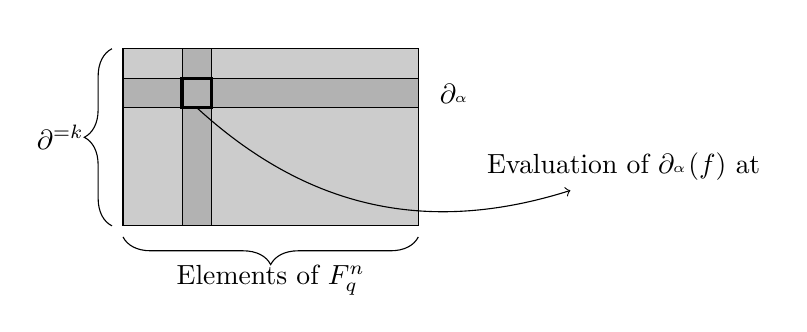
\begin{tikzpicture}[scale=0.75]
\draw[fill=black!20] (0,0) rectangle (5,3);

\draw[decorate,decoration={brace,amplitude=10pt,raise=4pt},yshift=0pt]
(0,0) -- (0,3);
\node[anchor=east] at (-0.5,1.5) {$\partial^{=k}$};
\draw[decorate,decoration={brace,amplitude=10pt,mirror, raise=4pt},yshift=0pt] 
(0,0) -- (5,0);
\node[anchor=north] at (2.5,-0.5) {Elements of $F_q^n$};

\draw[fill=black!30] (1,0) rectangle (1.5,3);
\node at (1.25,3.2) {$\veca$};

\draw[fill=black!30] (0,2) rectangle (5,2.5);
\node[anchor=west] at (5.2,2.2) {$\partial_{\vecx^\alpha}$};

\draw[very thick] (1,2) rectangle (1.5,2.5);

\node[anchor=west] at (6,1) {Evaluation of $\partial_{\vecx^\alpha}(f)$ at $\veca$}
edge[<-,bend left] (1.25,2);
\end{tikzpicture}

As seen in \autoref{chap:GK}, the measure $\CM{GK}_k$ was the rank of the above matrix (with a few columns removed).
Intuitively, we expect that if the rank of the \emph{coefficient} matrix is large, then the rank of the \emph{evaluation} matrix should also be large.
Sometimes, the evaluation perspective allows us to handle the circuit model better.
In a way, the proof of Grigoriev and Karpinski~\cite{grigoriev98} can be thought of as a formalization of this intuition for $\SPS$ circuits.
\\

A similar perspective can also be adopted for the dimension of shifted partial derivatives.
For the dimension of projected shifted partials however, this connection is not that clean.
Roughly speaking, throwing away non-multilinear monomials changes the evaluations of the shifted partials at points.
Formally, the multilinear projection of a polynomial $f$ can be interpreted as looking at the residue of $f \bmod \setdef{x_i^2}{i\in [n]}$, that is just replacing any $x_i^2$ by zero.
However this reduction does not work well with evaluations as $f(\veca)$ could be different from $(f \bmod \setdef{x_i^2}{i\in [n]})(\veca)$ for each $\veca \in \F^n$. 

Let us turn the question around and ask if we wish to understand the rank of the following matrix

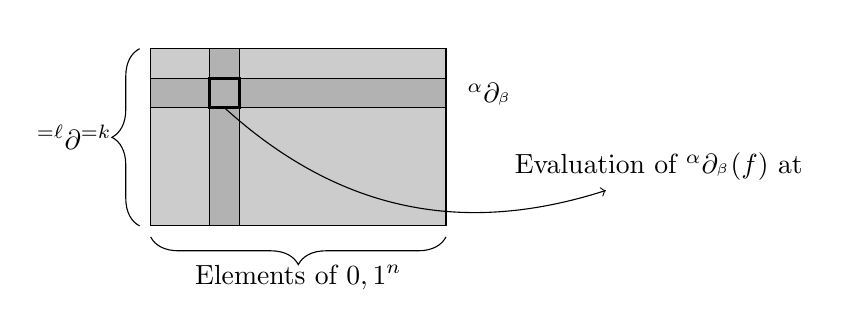
\begin{tikzpicture}[scale=0.75]
\draw[fill=black!20] (0,0) rectangle (5,3);

\draw[decorate,decoration={brace,amplitude=10pt,raise=4pt},yshift=0pt]
(0,0) -- (0,3);
\node[anchor=east] at (-0.5,1.5) {$\vecx^{=\ell}\partial^{=k}$};
\draw[decorate,decoration={brace,amplitude=10pt,mirror, raise=4pt},yshift=0pt] 
(0,0) -- (5,0);
\node[anchor=north] at (2.5,-0.5) {Elements of $\set{0,1}^n$};

\draw[fill=black!30] (1,0) rectangle (1.5,3);
\node at (1.25,3.2) {$\veca$};

\draw[fill=black!30] (0,2) rectangle (5,2.5);
\node[anchor=west] at (5.2,2.2) {$\vecx^{\alpha}\partial_{\vecx^\beta}$};

\draw[very thick] (1,2) rectangle (1.5,2.5);

\node[anchor=west] at (6,1) {Evaluation of $\vecx^\alpha\partial_{\vecx^\beta}(f)$ at $\veca$}
edge[<-,bend left] (1.25,2);
\end{tikzpicture}

\noindent
what is the \emph{coefficient} analogue of this measure?
Turns out, the answer is a different notion of projected shifted partial derivatives where the projection is not modulo $\setdef{x_i^2}{i\in [n]}$ but instead modulo $\setdef{x_i^2 - x_i}{i\in [n]}$.
It should be intuitively clear that as long as we are only interested in evaluations on $\set{0,1}^n$, the evaluation of  $f \bmod \setdef{x_i^2 - x_i}{i\in [n]}$ at $\veca\in \set{0,1}^n$ yields the same  as $f(\veca)$. 

What can we say about this modification of projected shifted partial derivatives? Is this also a measure that can give the homogeneous depth-$4$ lower bounds studied in \autoref{chap:d4hom}? Turns out the answer is indeed yes, and this perspective also allows one to generalize the lower bounds to homogeneous depth-$5$ circuits over finite fields (similar to Grigoriev-Karpinski) by Kumar and Saptharishi~\cite{KumarSapt15}. 

\section{Projected shifted partials via $\setdef{x_i^2-x_i}{i\in [n]}$}

The following definition is a little more general but would be useful later in this chapter. But for now, it would be useful to just consider $\mathcal{I} = \inangle{x_i^2 - x_i \;:\; i\in [n]}$. 

 \begin{definition}[PSDs with respect to $\mathcal{I}$] \label{defn:PSPD-ideal}
The \emph{projected shifted partial derivatives with respect to $\mathcal{I}$} for a polynomial $f$, denoted by $\Gamma_{k,\ell,\mathcal{I}}(f)$, is defined as 
\[
\Gamma^{\mathrm{PSD}}_{k,\ell,\mathcal{I}}(f) \spaced{:=} \dim \set{\inparen{\vecx^{=\ell} \cdot \partial^{=k}(f)} \bmod \mathcal{I}}.\qedhere
\]
\end{definition}
\noindent
In the setting where $\mathcal{I} = \inangle{x_i^2 - x_i\;:\; i\in [n]}$, every polynomial $f$, there is a unique multilinear polynomial $g$ for which $f = g \bmod \mathcal{I}$ and we shall refer to this $g$ by $f \bmod \mathcal{I}$. Thus, $\Gamma_{k,\ell,\mathcal{I}}(f)$ is the rank of the following matrix:

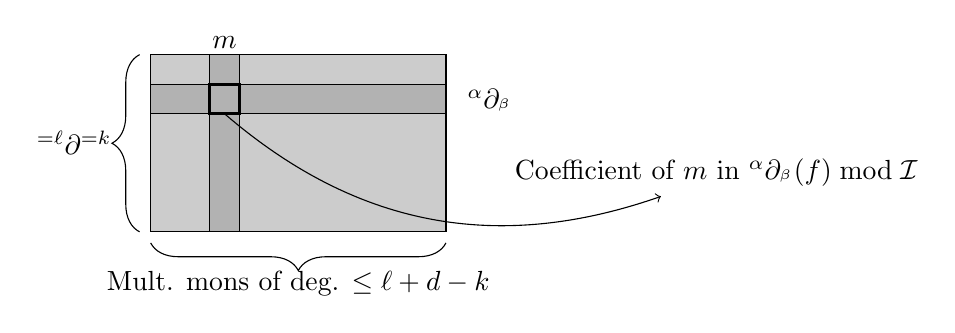
\begin{tikzpicture}[scale=0.75]
\draw[fill=black!20] (0,0) rectangle (5,3);

\draw[decorate,decoration={brace,amplitude=10pt,raise=4pt},yshift=0pt]
(0,0) -- (0,3);
\node[anchor=east] at (-0.5,1.5) {$\vecx^{=\ell}\partial^{=k}$};
\draw[decorate,decoration={brace,amplitude=10pt,mirror, raise=4pt},yshift=0pt] 
(0,0) -- (5,0);
\node[anchor=north] at (2.5,-0.5) {Mult. mons of deg. $\leq \ell + d - k$};

\draw[fill=black!30] (1,0) rectangle (1.5,3);
\node at (1.25,3.2) {$m$};

\draw[fill=black!30] (0,2) rectangle (5,2.5);
\node[anchor=west] at (5.2,2.2) {$\vecx^{\alpha}\partial_{\vecx^\beta}$};

\draw[very thick] (1,2) rectangle (1.5,2.5);

\node[anchor=west] at (6,1) {Coefficient of $m$ in $\vecx^\alpha\partial_{\vecx^\beta}(f) \bmod \mathcal{I}$}
edge[<-,bend left] (1.25,2);
\end{tikzpicture}

\noindent In \autoref{defn:PSPD}, we are essentially working with
$\mathcal{I} = \inangle{x_i^2 \;:\; i\in [n]}$ but working modulo other ideals is at times more useful.
In fact, there is a fairly large class of ideals $\mathcal{I}$ for which $f \bmod \mathcal{I}$ has a unique multilinear representative. But to make it applicable for lower bounds for homogeneous depth-$4$ circuits, we will need a mechanism to transform a ``low support polynomial'' to a ``low degree polynomial''. 

\begin{definition}[Support-to-degree ideals]
An ideal $\mathcal{I}$ is said to be a \emph{support-to-degree} ideal if there exist linear polynomials $\ell_1, \cdots, \ell_n$ such that
\[
\mathcal{I} \spaced{=} \inangle{x_i^2 - \ell_i(x_i) \;:\; i\in [n]}. \qedhere
\]
\end{definition}

\begin{observation}\label{obs:support-redn}
For any polynomial $f$ and a support-to-degree ideal $\mathcal{I}$, there is a unique multilinear polynomial $g$ such that $f = g \bmod\mathcal{I}$. 

Furthermore, if $f$ is a polynomial such that every monomial in $f$ depends on at most $r$ variables, then the unique multilinear polynomial $g = f \bmod\mathcal{I}$ in fact has degree at most $r$. 
\end{observation}
\begin{proof}
The proof follows immediately by repeatedly replacing $x_i^2$ by $\ell_i(x_i)$.
\end{proof}

As mentioned before, we would need the above more general definition in a later lower bound but for now it would help to just keep ideals such as $\inangle{x_i^2\;:\;i\in [n]}$ or $\inangle{x_i^2 - x_i\;:\;i\in [n]}$ in mind. \\

In order to check if \autoref{defn:PSPD-ideal} is a measure useful for homogeneous depth-$4$ circuits, we need to show two things --- (1) the measure is small for a small homogeneous depth-$4$ circuit (of low bottom support), and (2) the measure is large for an explicit polynomial.
These together would imply the practicability of dimension of projected shifted partials with respect to an arbitrary support-to-degree ideal.

The second claim would be easier to prove so let us address that first. 

\begin{lemma}[PSD wrt $\mathcal{I}$ for homogeneous polynomials]\label{lem:PSD-I-lowerbound} Let $f$ be any homogeneous polynomial of degree $d$. For any choice of $k,\ell$ and any support-to-degree ideal $\mathcal{I}$, we have
\[
\Gamma^{\mathrm{PSD}}_{k,\ell,\mathcal{I}}(f) \spaced{\geq} \Gamma^{\mathrm{PSD}}_{k,\ell}(f).
\]
\end{lemma}
\begin{proof}
  Let $g \in \vecx^{=\ell} \cdot \partial^{=k}(f)$.
The main difference between $g \bmod \inangle{x_i^2\;:\; i \in [n]}$ and $g \bmod\mathcal{I}$ is just that the first projection just zeros out any non-multilinear monomial of degree $\ell + d -k$ whereas $g \bmod\mathcal{I}$ reduces non-multilinear monomials to lower degree monomials.
Hence, $g \bmod\inangle{x_i^2\;:\; i \in [n]}$ is just $g \bmod \mathcal{I}$ but just restricted to the multilinear monomials of degree $\ell + d - k$. 
Thus it follows that the rank of $\inparen{\vecx^{=\ell} \partial^{=k}g} \bmod\mathcal{I}$ is lower bounded by the rank of $\inparen{\vecx^{=\ell} \partial^{=k}g} \bmod\inangle{x_i^2\;:\; i \in [n]}$.
\end{proof}

We now want to show that if $C$ is a homogeneous depth-$4$ circuit with bottom support at most $r = O(\sqrt{d})$, then we can give a good upper bound for $\Gamma^{\mathrm{PSD}}_{k,\ell,\mathcal{I}}(C)$. 

\begin{lemma}[PSD wrt $\mathcal{I}$ for a hom. $\SPSP$ circuit]\label{lem:PSPD-I-upperbound} Let $C$ be a homogeneous $\SPSP$ computing an $n$-variate degree $d$ polynomial of top fan-in $s$ and bottom support bounded by $r$. Then for any choice of $k,\ell$ and any support-to-degree ideal $\mathcal{I}$ we have
\[
\Gamma^{\mathrm{PSD}}_{k,\ell,\mathcal{I}} \spaced{\leq} s \cdot \binom{3(d/r) + 1}{k} \cdot \binom{n}{\ell + kr}
\]
\end{lemma}
\begin{proof}
  Let us consider a single summand $T = Q_1 \cdots Q_m$ of $C$.
We shall partition this set into those polynomials $Q_1,\cdots, Q_a$ of degree at most $r$, and polynomials $Q_1',\cdots, Q_b'$ of degree more than $r$. By homogeneity of $C$, we know that $b \leq d/r$. Since some of the $Q_i$s could have very small degree, $a$ could potentially be as large as $d$. To handle this, if we find any $Q_i$ and $Q_j$ both of degree at most $r/2$, we shall replace them by their product. This ensures that all $Q_i$s have degree more than $r/2$ except perhaps one. Hence, (reusing some symbols) we can write $T$ as
\[
T \spaced{=} \tilde{Q}_1 \cdots \tilde{Q}_a \;\cdot\; Q_1' \cdots Q_b'
\]
where each $a \leq 2(d/r) + 1$, $b \leq (d/r)$, each $Q_i$ has degree at most $r$ and every monomial in a $Q_i'$ depends on at most $r$ variables. For brevity, we shall use the notation $\tilde{Q}_A$ to denote $\prod_{i\in A} \tilde{Q}_i$, and similarly $Q_B'$ to denote $\prod_{i\in B} Q_i'$. 

Let $\partial_{\vecx^\alpha}(T)$ be a $k$-th order partial derivative of $T$. By the chain rule of differentiation,
\begin{eqnarray*}
\partial_{\vecx^\alpha}(T) & \in & \mathrm{span}\setdef{ \partial_{\vecx^\beta}(\tilde{Q}_A) \cdot \partial_{\vecx^\gamma}(Q_B') \cdot \tilde{Q}_{\overline{A}} \cdot Q_{\overline{B}}'}{\begin{array}{c} \vecx^{\alpha} = \vecx^\beta \cdot \vecx^\gamma\\ |A| + |B| \leq k  \end{array}}\\
 & \subseteq & \mathrm{span}\setdef{ \vecx^{\leq k(r - 1)} \cdot \partial_{\vecx^\gamma}(Q_B') \cdot \tilde{Q}_{\overline{A}} \cdot Q_{\overline{B}}'}{\begin{array}{c} \vecx^{\alpha} = \vecx^\beta \cdot \vecx^\gamma\\ |A| + |B| \leq k  \end{array}}\\
\implies \vecx^{=\ell} \cdot \partial_{\vecx^\alpha}(T) & \subseteq & \mathrm{span}\setdef{ \vecx^{\leq \ell + k(r - 1)} \cdot \partial_{\vecx^\gamma}(Q_B') \cdot \tilde{Q}_{\overline{A}} \cdot Q_{\overline{B}}'}{\begin{array}{c} \vecx^{\alpha} = \vecx^\beta \cdot \vecx^\gamma\\ |A| + |B| \leq k  \end{array}}
\end{eqnarray*}
We now have to look at $\vecx^{=\ell} \cdot \partial_{\vecx^\alpha}(T) \bmod\mathcal{I}$ and for that notice that $Q_B'$ is a product of polynomials of low-support, that is each monomial $Q_i'$ depends on at most $\sqrt{d}$ variables. Therefore, by applying the product rule on $\partial_{\vecx^{\gamma}}(Q_B')$, we know that this can be written as a linear combination of products of low-support polynomials. By \autoref{obs:support-redn}, every polynomial $f$ of support at most $r$ there is a unique multilinear polynomial $g = f\bmod \mathcal{I}$ of degree at most $r$. Hence, we get that
\begin{eqnarray*}
\vecx^{=\ell} \cdot \partial_{\vecx^\alpha}(T) \bmod\mathcal{I} & \subseteq& \mathrm{span}\setdef{ \vecx^{\leq \ell + k(r - 1)} \cdot \vecx^{\leq k(r)} \cdot \tilde{Q}_{\overline{A}} \cdot Q_{\overline{B}}'}{\begin{array}{c} \vecx^{\alpha} = \vecx^\beta \cdot \vecx^\gamma\\ |A| + |B| \leq k  \end{array}} \bmod \mathcal{I}\\
& = & \mathrm{span}\setdef{ \vecx^{\leq \ell + kr} \cdot \tilde{Q}_{\overline{A}} \cdot Q_{\overline{B}}'}{\begin{array}{c} \vecx^{\alpha} = \vecx^\beta \cdot \vecx^\gamma\\ |A| + |B| \leq k  \end{array}} \bmod \mathcal{I}.
\end{eqnarray*}
\noindent
Therefore, an upper bound on $\set{\vecx^{=\ell} \partial^{=k}(T) \bmod \mathcal{I}}$ is 
\[
\binom{2(d/r) + 1 + (d/r)}{k} \cdot \binom{n}{\ell + kr} \cdot n
\]
\noindent
Hence, if $C = T_1 + \cdots + T_s$, then by sub-additivity we get
\[
\Gamma^{\mathrm{PSD}}_{k,\ell,\mathcal{I}}(C) \spaced{=} s \cdot \binom{3(d/r) + 1}{k} \cdot \binom{n}{\ell + kr} \cdot n.\qedhere
\]
\end{proof}

\noindent
The bound above is almost the same as in \autoref{lem:upper-bound-low-supp} and the difference is only $\exp(O(d/r))$ due to the first binomial coefficient above. \autoref{lem:PSD-I-lowerbound} and 
\autoref{lem:d4hom-goldilocks-LB} yields a lower bound for $\Gamma^{\mathrm{PSD}}_{k,\ell,\mathcal{I}}(\NW)$ as well. \\

What did we gain by looking at $\Gamma^{\mathrm{PSD}}_{k,\ell,\mathcal{I}}$ at the end of all this?
The key point is makes it easier to look at the evaluation perspective for such measures when the ideal $\mathcal{I}$ \emph{cooperates} with the evaluation operation.
A concrete instance of this was the lower bound by Kumar and Saptharishi~\cite{KumarSapt15} for homogeneous depth five circuits over finite fields.

\section{Lower bounds for depth five circuits over finite fields}








%%% Local Variables: 
%%% mode: latex
%%% TeX-master: "main"
%%% End: 
